\documentclass[tikz, border=10pt]{standalone}
\usepackage{tikz}
\usetikzlibrary{arrows.meta, positioning, shapes.geometric, calc}

\begin{document}
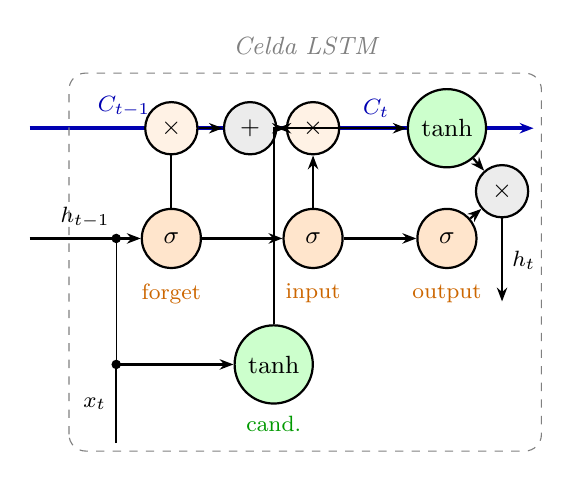
\begin{tikzpicture}[
    gate/.style={draw, circle, minimum size=0.75cm, thick, fill=orange!20},
    op/.style={draw, circle, minimum size=0.65cm, thick, fill=gray!15},
    tanh/.style={draw, circle, minimum size=0.75cm, thick, fill=green!20},
    arr/.style={-{Stealth[length=5pt]}, thick},
    font=\small,
    lbl/.style={font=\footnotesize}
]

% ---- Cell state (top horizontal line) ----
\draw[arr, line width=1.4pt, blue!70!black]
    (-0.8, 3.2) -- node[above, lbl, blue!70!black]{$C_{t-1}$} (1.6, 3.2)
                -- node[above, lbl, blue!70!black]{$C_t$}      (5.6, 3.2);

% ---- Forget gate (left) ----
\node[gate] (fg) at (1.0, 1.8) {$\sigma$};
\node[lbl, text=orange!80!black] at (1.0, 1.1) {forget};
\draw[arr] (fg) -- (1.0, 3.2);  % output up to cell state multiply
\node[op, fill=orange!10] (mulf) at (1.0, 3.2) {$\times$};

% ---- Input gate + candidate ----
\node[gate] (ig) at (2.8, 1.8) {$\sigma$};
\node[lbl, text=orange!80!black] at (2.8, 1.1) {input};
\node[tanh] (cand) at (2.3, 0.2) {$\tanh$};
\node[lbl, text=green!60!black] at (2.3, -0.55) {cand.};

\node[op, fill=orange!10] (mul_i) at (2.8, 3.2) {$\times$};
\node[op] (add_c) at (2.0, 3.2) {$+$};

\draw[arr] (ig) -- (mul_i);
\draw[arr] (cand) -- (2.3, 3.2) -- (mul_i);
\draw[arr] (mul_i) -- (add_c);
\draw[arr] (mulf) -- (add_c);

% ---- Output gate ----
\node[gate] (og) at (4.5, 1.8) {$\sigma$};
\node[lbl, text=orange!80!black] at (4.5, 1.1) {output};
\node[tanh] (tanh_out) at (4.5, 3.2) {$\tanh$};
\node[op] (mul_o) at (5.2, 2.4) {$\times$};

\draw[arr] (og) -- (mul_o);
\draw[arr] (tanh_out) -- (mul_o);
\draw[arr] (add_c) -- (tanh_out);

% ---- h_t output ----
\draw[arr] (mul_o) -- node[right, lbl]{$h_t$} (5.2, 1.0);

% ---- Input h_{t-1} and x_t ----
\draw[arr] (-0.8, 1.8) -- node[above, lbl]{$h_{t-1}$} (fg);
\draw[arr] (fg) -- (ig);
\draw[arr] (ig) -- (og);

\draw[arr] (0.3, -0.8) -- node[left, lbl]{$x_t$} (0.3, 0.2) -- (cand);
\draw (0.3, 0.2) -- (0.3, 1.8);
\filldraw[black] (0.3, 0.2) circle (1.5pt);
\filldraw[black] (0.3, 1.8) circle (1.5pt);

% ---- Border box ----
\draw[dashed, rounded corners=6pt, gray]
    (-0.3, -0.9) rectangle (5.7, 3.9);
\node[gray, font=\small\itshape] at (2.7, 4.25) {Celda LSTM};

\end{tikzpicture}
\end{document}
